%-------------------------------------------------------------------------------
% Autores: I. R. Pagnossin e Centro de Ensino e Pesquisa Aplicada.
%
% Este material é parte integrante do curso "Usando LaTeX; pensando em TeX" e é
% distribuido pelos autores segundo a licença Creative Commons 2.5 Brasil
% (atribuição/não-comercial/redistribuição segundo a mesma licença).
%
% This material is part of the course "Usando LaTeX; pensando em TeX".
% It is distributed according to the license Creative Commons 2.5 Brazil
% (attribution/non-comercial use/share alike the same license).
%-------------------------------------------------------------------------------
\newif\ifhandout
%\handouttrue  % Descomente se for para gerar a versão para IMPRESSÃO.
\handoutfalse % Descomente se for para gerar a versão para APRESENTAÇÃO

%-------------------------------------------------------------------------------
\ifhandout
  \documentclass[handout,10pt]{beamer}
  \mode<handout>
\else
	\documentclass[10pt,hyperref={pdfpagelabels=false}]{beamer}
	\mode<presentation>
\fi

	\usepackage[utf8]{inputenc}
	\usepackage[brazil]{babel}	
	\usepackage{graphicx}
	\usepackage{listings}
	\usepackage{amsmath}
	\usepackage{tikz}	
	\usepackage[squaren]{SIunits}	
	\usepackage{fancybox}
	\usepackage{array}
	\usepackage{colortbl}		
	\usepackage{bookman}
	\usepackage{fancybox}
	\usepackage{booktabs}
	\usepackage{helvet}
	\usepackage{lipsum}
	\usepackage{tabularx}
	\usepackage{calc}
	\usepackage{colortbl}
		
	\ifhandout
		\usepackage{pgfpages}
		\pgfpagesuselayout{2 on 1}[a4paper,border shrink=5mm]
	\fi

	% Bibliotecas TikZ e PGF necessárias
	\usetikzlibrary{shapes.symbols}
	\usepgflibrary{shapes.misc}
	\usetikzlibrary{calc}
	
	% Configurações pessoais
	% Configurações personalizadas do código LaTeX.	
\lstnewenvironment{LaTeXcode}{
	\setlength{\abovecaptionskip}{0pt}	
	\lstset{language=[LaTeX]TeX}
	\lstset{%
		basicstyle=\footnotesize\ttfamily,  % Global
		keywordstyle=\color{blue}\bfseries, % Comandos
		identifierstyle=,                   % Texto
		stringstyle=,                       % Strings 
		commentstyle=\color{gray},          % Comentários
		showstringspaces=false,             % Espaços
		rulecolor=\color{gray},             % Linha da caixa
	}
	\lstset{emph={setlength,includegraphics,psfrag,subfigure},emphstyle={\color{blue}\bfseries}}
}% Abrindo o ambiente.
{}% Fechando o ambiente.
	
\newcommand{\digite}[1]{{\fontfamily{cmss}\fontseries{bx}\selectfont#1}}	
\newcommand{\cs}[1]{{\normalfont\textbackslash\color{blue!50!black}#1}}
\newcommand{\pkg}[1]{{\normalfont\sffamily\color{orange}#1}}
\newcommand{\env}[1]{{\normalfont\sffamily\color{green!50!black}#1}}
\let\comando=\cs
\let\package=\pkg
\let\ambiente=\env
\newcommand{\foreign}[1]{{\textsl{#1}}}


	\newcounter{exercicio}	
	\newenvironment{exercicio}{%
		\refstepcounter{exercicio}%
		\penalty-200
		\noindent\colorbox{blue!60!black}{\makebox[\columnwidth-\fboxsep*2][c]{\textbf{\color{white}Exercício~\theexercicio}}}\smallskip
	}{\par\medskip}
		

\newcommand{\bibtex}{\textsc{Bib}\TeX}

\newenvironment<>{atividade}[1]{%
\begin{actionenv}#2%
\begin{exampleblock}{{Atividade #1}}%
}
{%
\end{exampleblock}%
\end{actionenv}%
}


	% Path das figuras, relativo a esta pasta.
	\graphicspath{{../arquivos_comuns/figuras/}{./figuras/}}

	% Modelo da apresentação	
	\usetheme{Frankfurt}
	\usefonttheme{serif,structurebold}
	%\setbeamercovered{transparent}		
		
	% Metadados do arquivo PDF.
	\hypersetup{
		pdftitle={Figuras externas},
		pdfauthor={Dr. Ivan R. Pagnossin},
		pdfsubject={LaTeX},
		pdfkeywords={TeX,LaTeX}
	}

	% Título, autores e instituição.
	\title{Figuras externas}
	\author{\textbf{Prof.:} Ivan R. Pagnossin\and \textbf{Tutora:} Juliana Giordano}
	\institute{%
		Coordenadoria de Tecnologia da Informação\\
		Centro de Ensino e Pesquisa Aplicada}
	\logo{
\includegraphics[width=0.25\textwidth]{LogotipoCursoLaTeX_v3_pequeno}}
	\date{}
	
	\newcommand{\scalefactor}{7}
	\tikzset{box/.style={color=#1,thick},box/.default=red}
	\tikzset{letter/.style={color=#1,inner sep=0pt},letter/.default=gray!50}
	\tikzset{baseline/.style={color=#1,thin},baseline/.default=blue}
		
	\newsavebox{\meuparbox}
	
\begin{document}
%-------------------------------------------------------------------
\begin{frame}[c,label=titulo]
	\centering	
	
	
\includegraphics[width=0.8\textwidth]{LogotipoCursoLaTeX_v2}

	\titlepage
\end{frame}
%-------------------------------------------------------------------
\logo{} % <-- O logotipo não aparecerá mais a partir daqui.
\setbeamertemplate{background canvas}{%
		
\includegraphics[width=\paperwidth,height=\paperheight,keepaspectratio=false]{leao-pensador-wattermark.png}
}
%-------------------------------------------------------------------
\section{Inclusão de figuras externas}
\subsection{Sintaxe do comando {\ttfamily\textbackslash includegraphics}}
\begin{frame}[fragile]
	\frametitle{Figuras externas: {\ttfamily\textbackslash includegraphics}}
	\framesubtitle{O pacote \pkg{graphicx}}
	
	\begin{block}<1->{}
		\centering
		\cs{includegraphics}\verb|[|%
			\textit{opções}%
		\verb|]{|%
			\textit{figura}%
		\verb|}|
	\end{block}
	
	\begin{columns}
		\column[c]{0.5\textwidth}
		\begin{atividade}<2->{1 e 2}
			\begin{LaTeXcode}
				\noindent\hrulefill\
				\includegraphics{figura}
				\hrulefill
			\end{LaTeXcode}
		\end{atividade}
		
		\medskip
		
		\begin{uncoverenv}<3->
			\hrulefill\
			
\includegraphics[width=0.5\textwidth]{Tei-Gi}\
			\hrulefill
		\end{uncoverenv}
		
		\column[c]{0.4\textwidth}		
		\begin{uncoverenv}<4->
			\begin{tabular}{cccc}
				\toprule
				Figura & \multicolumn{3}{c}{Doc. final} \\
				\cmidrule{2-4}
				& \texttt{dvi} & \texttt{ps} & \texttt{pdf} \\
				\midrule
				\texttt{\textcolor{blue}{eps}} & \checkmark & \checkmark \\
				\texttt{jpg} & & & \checkmark \\
				\texttt{png} & & & \checkmark \\
				\texttt{\textcolor{blue}{pdf}} & & & \checkmark \\
				\bottomrule
			\end{tabular}	
		\end{uncoverenv}
		
		\begin{block}<5->{Exercício 1\hspace*{\stretch{1}}\hyperlink{respostas}{\footnotesize\textbf{(resposta)}}}
			Identifique a origem dos dois espaços ao lado da figura
		\end{block}
	\end{columns}
	
\end{frame}
%-------------------------------------------------------------------
\subsection{Opções do comando {\ttfamily\textbackslash includegraphics}}
\begin{frame}[fragile]
	\frametitle{Opções do comando {\ttfamily\textbackslash includegraphics}}
	\framesubtitle{O esquema de pares chave-valor}
	
	O (único) argumento opcional de \cs{includegraphics} utiliza o esquema de
	\emph{pares	chave-valor}, separados por vírgula:
		
	\begin{block}<1->{}
		\centering
		\(\textcolor{green!50!black}{chave} = \textcolor{red}{valor}\)\uncover<2->{,
		\(\textcolor{green!50!black}{chave} = \textcolor{red}{valor}\),
		\dots,}
		\uncover<3->{\(\textcolor{green!50!black}{chave} = \textcolor{red}{valor}\)}
	\end{block}
	
	\vfill
	
	\uncover<4->{Exemplos:}
	\begin{itemize}\ttfamily
		\item<4-> \cs{includegraphics}[%
			\textcolor{green!50!black}{scale}=\textcolor{red}{0.5}]\{\dots\}
			
		\item<5-> \cs{includegraphics}[%
			\textcolor{green!50!black}{width}=\textcolor{red}{5cm},%
			\textcolor{green!50!black}{height}=\textcolor{red}{5cm}]\{\dots\}
			
		\item<6-> \cs{includegraphics}[%
			\textcolor{green!50!black}{angle}=\textcolor{red}{25},%
			\textcolor{green!50!black}{draft}=\textcolor{red}{true}]\{\dots\}
			
		\item<7-> \cs{includegraphics}[%
			\textcolor{green!50!black}{trim}=\textcolor{red}{1 2 3 4},\textcolor{green!50!black}{clip}]\{\dots\}
			
		\item<7-> \normalfont Veja outras opções na documentação do pacote
	\end{itemize}
	
	\vfill
	
	\scriptsize
	\begin{uncoverenv}<8->
		\textbf{obs.:} devido à flexibilidade do esquema de pares chave-valor,
		muitos pacotes o adotam em detrimento do restrito esquema original, de 
		palavras-chave separadas por vírgula.
	\end{uncoverenv}
	
\end{frame}
%-------------------------------------------------------------------
\begin{frame}[fragile]
	\frametitle{Opções do comando {\ttfamily\textbackslash includegraphics}}

	\begin{columns}
		\centering
	
		\column{0.45\textwidth}		
		
		\begin{atividade}{3}
			\begin{LaTeXcode}
			
\includegraphics[
			  width  = 2cm,
			  height = 1cm
			  ]{Tei-Gi}\par
				
			
\includegraphics[
			  width  = 2cm,
			  height = 1cm
			  keepaspectratio=true
			  ]{Tei-Gi}\par
							
			
\includegraphics[
			  angle = 70]{Tei-Gi}
			  
			
\includegraphics
			  [draft=true]{Tei-Gi}
			\end{LaTeXcode}		
		\end{atividade}
		
		\column{0.45\textwidth}	
		\centering
	
		
\includegraphics[			
			width  = \textwidth,
			height = 1cm
			]{Tei-Gi}
		
		\medskip
		
		
\includegraphics[
			width  = 2cm,
			height = 1cm,
			keepaspectratio=true
			]{Tei-Gi}\par
			
		\medskip
		
		
\includegraphics[
		  width  = 2cm,
		  height = 2cm,		
		  angle  = 70]{Tei-Gi}
			
		\medskip
		
		
\includegraphics[
			width  = 2cm,
			height = 2cm,
			draft  = true]{Tei-Gi}
							
	\end{columns}
\end{frame}
%-------------------------------------------------------------------
\section{Transformações de figuras/caixas}
\begin{frame}[fragile]
	\frametitle{Transformações de figuras/caixas}

	\begin{block}<1->{}
		\cs{rotatebox}\verb|[|%
			\textit{opções}%
		\verb|]{|%
			\textit{ângulo}%
		\verb|}{|%
			\textit{\textbf{caixa}}%
		\verb|}|
		
		\medskip
		
		\scriptsize
		\textbf{opções:} \texttt{origin}, \texttt{x}, \texttt{y}, \texttt{units}.
	\end{block}
		
	\begin{block}<2->{}	
		\cs{resizebox}\verb|{|%
			\textit{largura}%
		\verb|}{|%
			\textit{altura}%
		\verb|}{|%
			\textit{\textbf{caixa}}%
		\verb|}|
		
		\medskip
		
		\scriptsize
		\textbf{obs.:} se você definir apenas uma das dimensões e passar ! 
		(exclamação) como argumento da outra, ela será redimensionada de modo a
		manter a relação entre a altura e a largura da caixa.
	\end{block}
		
	\begin{block}<3->{}
		\cs{scalebox}\verb|{|%
			\textit{fator horizontal}%
		\verb|}[|%
			\textit{fator vertical}%
		\verb|]{|%
			\textit{\textbf{caixa}}%
		\verb|}|
	\end{block}
	
	\begin{block}<4->{}
		\cs{reflectbox}\verb|{|%
			\textit{\textbf{caixa}}%
		\verb|}|
	\end{block}

	\begin{atividade}<5->{4}
		Experimente os comandos acima.
	\end{atividade}
	
\end{frame}
%-------------------------------------------------------------------
\newsavebox{\compassbox}
\savebox{\compassbox}{
\includegraphics[width=1cm]{rosa_dos_ventos}}
\newcommand{\compass}{\usebox{\compassbox}}

\begin{frame}[fragile]
	\frametitle{Cuidado ao rotacionar caixas}
		
	\begin{center}
		\begin{actionenv}<1->
			\begin{tikzpicture}
			\node [rectangle,rounded corners=1mm,minimum size=7mm,very thick,
				draw=red!30, top color=red!20,bottom color=white!20]
				{\textbf{Caixas \textbf{não} rodam; seu conteúdo sim}};
			\end{tikzpicture}
		\end{actionenv}	
	\end{center}
					
	\vfill
	
	\setlength{\fboxsep}{0pt}
		
	\pause
	
	\hrulefill
	{\color{gray!50}
	\fbox{\rotatebox{0}{\color{red!50}{%
		\compass}}}}%
	\hrulefill
	{\color{gray!50}
	\fbox{\rotatebox{60}{\color{red!50}\fbox{%
		\compass}}}}%
	\hrulefill
	{\color{gray!50}
	\fbox{\rotatebox{120}{\color{red!50}\fbox{%
		\compass}}}}%
	\hrulefill
	{\color{gray!50}
	\fbox{\rotatebox{180}{\color{red!50}{%
		\compass}}}}%
	\hrulefill
	{\color{gray!50}
	\fbox{\rotatebox{240}{\color{red!50}\fbox{%
		\compass}}}}%
	\hrulefill
		
	\pause
	
	\vfill	
	
	\hrulefill
	{\color{gray!50}
	\fbox{\rotatebox[origin=c]{0}{\color{red!50}{%
		\compass}}}}%
	\hrulefill
	{\color{gray!50}
	\fbox{\rotatebox[origin=c]{60}{\color{red!50}\fbox{%
		\compass}}}}%
	\hrulefill
	{\color{gray!50}
	\fbox{\rotatebox[origin=c]{120}{\color{red!50}\fbox{%
		\compass}}}}%
	\hrulefill
	{\color{gray!50}
	\fbox{\rotatebox[origin=c]{180}{\color{red!50}{%
		\compass}}}}%
	\hrulefill
	{\color{gray!50}
	\fbox{\rotatebox[origin=c]{240}{\color{red!50}\fbox{%
		\compass}}}}%
	\hrulefill
				
\end{frame}
%-------------------------------------------------------------------
\section{Figuras flutuantes}
\subsection{O problema das caixas flutuantes}
\begin{frame}[fragile]
	\frametitle{Caixas flutuantes}
	\framesubtitle{ou \foreign{floats}}
	
	Às vezes a figura/tabela não cabe onde foi colocada. Nesses casos, utiliza-se
	o conceito de elementos flutuantes (caixas, no \LaTeX):
	
	\begin{block}<1->{}
		\centering
		\cs{begin}\verb|{figure}[|%
			\textit{posição \textbf{preferida}}%
		\verb|]|\dots
	\end{block}
	
	\small
	\begin{columns}
		\column[t]{0.47\textwidth}
		\uncover<2->{onde \textit{posição preferida} pode ser:}
		\begin{itemize}
			\item<2->[\texttt{h}] aqui (\foreign{here})
			\item<3->[\texttt{t}] início da página (\foreign{top})
			\item<4->[\texttt{b}] final da página (\foreign{bottom})
			\item<5->[\texttt{p}] página à parte (\foreign{page})
			\item<6->[\texttt{H}] aqui ``enfático''
		\end{itemize}
	
		\column[t]{0.5\textwidth}
		\uncover<7->{Regras:}
		\begin{enumerate}
			\item<7-> Após \cs{includegraphics}
			\item<8-> Em ordem de inserção
			\item<9-> Apenas uma posição
			\item<10-> Para \texttt{ht}, \texttt{h} tem preferência
			\item<11-> \cs{clearpage},\\ \cs{cleardoublepage} ou\\
				\cs{end}\verb|{document}|
		\end{enumerate}
	\end{columns}
		
\end{frame}
%-------------------------------------------------------------------
\subsection{Exemplo}
\begin{frame}[fragile]
	\frametitle{Caixas flutuantes}
	\framesubtitle{ou \foreign{floats}}

	\begin{atividade}<1->{5}
		Uma figura flutuante completa, com legenda e rótulo (para a referência 	
		cruzada):
	
		\begin{LaTeXcode}
			\begin{figure}[htb]
			  \centering
			  
\includegraphics[height=0.2\textheight]{Tei-Gi}
			  \caption{o Tei-Gi ou In Yang, símbolo
			    de equanimidade.}
			  \label{fig:tei-gi}
			\end{figure}
		\end{LaTeXcode}
	\end{atividade}
	
\end{frame}
%-------------------------------------------------------------------
\section{Figuras e legendas lado a lado}
\begin{frame}[fragile]
	\frametitle{Figuras e legendas lado a lado}
	
	\begin{atividade}{6}
		\begin{LaTeXcode}
			\begin{figure}
			  \begin{minipage}[b]{0.4\textwidth}
			    
\includegraphics[width=\textwidth]{./figuras/Tei-Gi}
			  \end{minipage}\hfill
			  \begin{minipage}[b]{0.5\textwidth}
			    \caption{legenda da figura, colocada ao lado dela através
			             de duas minipáginas.}
			    \label{fig:minipage}
			  \end{minipage}
			\end{figure}
		\end{LaTeXcode}
	\end{atividade}
	
	\begin{block}<2->{Exercício 2\hspace*{\stretch{1}}\hyperlink{respostas}{\footnotesize\textbf{(resposta)}}}
		Coloque duas figuras lado a lado, com suas respectivas legendas abaixo delas.
	\end{block}
	
\end{frame}
%-------------------------------------------------------------------
\section{Sub-figuras: o pacote subfigure}
\begin{frame}[fragile]
	\frametitle{Sub-figuras}
	\framesubtitle{O pacote \pkg{subfigure}}
	
	\begin{block}<1->{}
		\centering
		\cs{subfigure}[\textit{legenda curta}][\textit{legenda longa}]\{\textit{caixa}\}
	\end{block}
	
	\begin{atividade}<2->{7A e 7B}
		\small
		\begin{LaTeXcode}
			\begin{figure}[tb]
			  \hfill
			  \subfigure[Esta é a legenda da figura à esquerda]
			    {\label{fig:figA}%
			     
\includegraphics[width=0.45\textwidth]{Tei-Gi}}%			  
			  \hfill
			  \subfigure[Esta é a legenda da figura à direita]
			    {\label{fig:figB}%
			     
\includegraphics[width=0.45\textwidth]{Tei-Gi}}%
			  \hspace*{\fill} % <-- Por que não \hfill?
			
			  \caption{esta é a legenda comum às duas figuras.}
			  \label{fig:figAeB}
			\end{figure}
		\end{LaTeXcode}
	\end{atividade}
	
\end{frame}
%-------------------------------------------------------------------
\section{Substituição de texto em figuras EPS: o pacote psfrag}
\begin{frame}[fragile]
	\frametitle{Substituição de texto em figuras EPS}
	\framesubtitle{O pacote \pkg{psfrag}}
	
	\begin{block}<1->{}
		\begin{tabbing}
		\cs{psfrag}\=\kill
		\cs{psfrag}\>\{\textit{texto original}\}\\
		  \>[\textit{alinhamento do texto na figura}]\\
		  \>[\textit{alinhamento do texto do documento}]\\
		  \>\{\textit{texto final}\}
		\end{tabbing}
		  
		\footnotesize\textbf{obs.:} os alinhamentos podem ser \texttt{c} (\foreign{center}), \texttt{l} (\foreign{left}) ou \texttt{r} (\foreign{right}).
	\end{block}
	
	\begin{atividade}<2->{8}
		\begin{LaTeXcode}
			\begin{figure}
			  \centering
			  \psfrag{Texto na figura}[c][c]
			    {$\displaystyle\Gamma(z) = \int_0^\infty ...$}
			  
\includegraphics[width=0.5\textwidth]{./figuras/Tei-Gi.eps}
			  \caption{a substituição de texto só funciona com figuras EPS.}
			\end{figure}
		\end{LaTeXcode}
	\end{atividade}
	
	\uncover<2->{\begin{center}
		\footnotesize
		\textbf{Atenção:} você deve utilizar o perfil de compilação\\ $\text{\LaTeX} \Rightarrow \text{PS}$ ou $\text{\LaTeX} \Rightarrow \text{PS} \Rightarrow \text{PDF}$.
	\end{center}}
\end{frame}
%-------------------------------------------------------------------
\section{Ferramentas para a produção de figuras}
\subsection{Aplicativos e linguagens}
\begin{frame}
	\frametitle{Ferramentas para a produção de figuras}
	\framesubtitle{e as extensões dos arquivos que produzem}
		
	\begin{tabular}{lcccccc}
		\toprule
		\foreign{Software}      & EPS        & PSTricks   & TikZ       & PDF        & PNG        & JPG       \\
		\multicolumn{7}{c}{\cellcolor{red!50!black}\textbf{\textcolor{white}{Mapas de bits}}}\\
		\href{http://www.adobe.com/br/products/photoshop/photoshop/}{Adobe Photoshop}
		         & \checkmark &            &            & \checkmark & \checkmark & \checkmark\\
		\href{http://www.gimp.org/}{Gimp}
		                    &            &            &            &            & \checkmark & \checkmark\\
		\multicolumn{7}{c}{\cellcolor{red!50!black}\textbf{\textcolor{white}{Desenhos}}}\\
		\href{http://www.corel.com.br/}{Corel Draw}
		              & \checkmark &            &            & \checkmark & \checkmark & \checkmark\\
		\href{http://www.adobe.com/br/products/illustrator/}{Adobe Illustrator}
		       & \checkmark &            &            & \checkmark & \checkmark & \checkmark\\
		\href{http://www.inkscape.org/}{Inkscape}
		                & \checkmark & \checkmark &            & \checkmark &            &           \\
		\href{http://www.geogebra.org/cms/}{Geogebra}
		                & \checkmark & \checkmark\\
		\href{http://projects.gnome.org/dia/}{DIA} (diagramas)
		         & \checkmark &            &            &            & \checkmark &           \\
		\multicolumn{7}{c}{\cellcolor{red!50!black}\textbf{\textcolor{white}{Gráficos}}}\\
		\href{http://www.originlab.com/}{Origin}                  & \checkmark &            &            & \checkmark & \checkmark & \checkmark\\
		\href{http://glx.sourceforge.net/}{GLE}                     & \checkmark &            &            & \checkmark & \checkmark & \checkmark\\
		\href{http://www.gnuplot.info/}{Gnuplot}                 &            &            &            &            & \checkmark &           \\
		\bottomrule
	\end{tabular}
\end{frame}
%-------------------------------------------------------------------
\newsavebox\exemploA
\savebox\exemploA{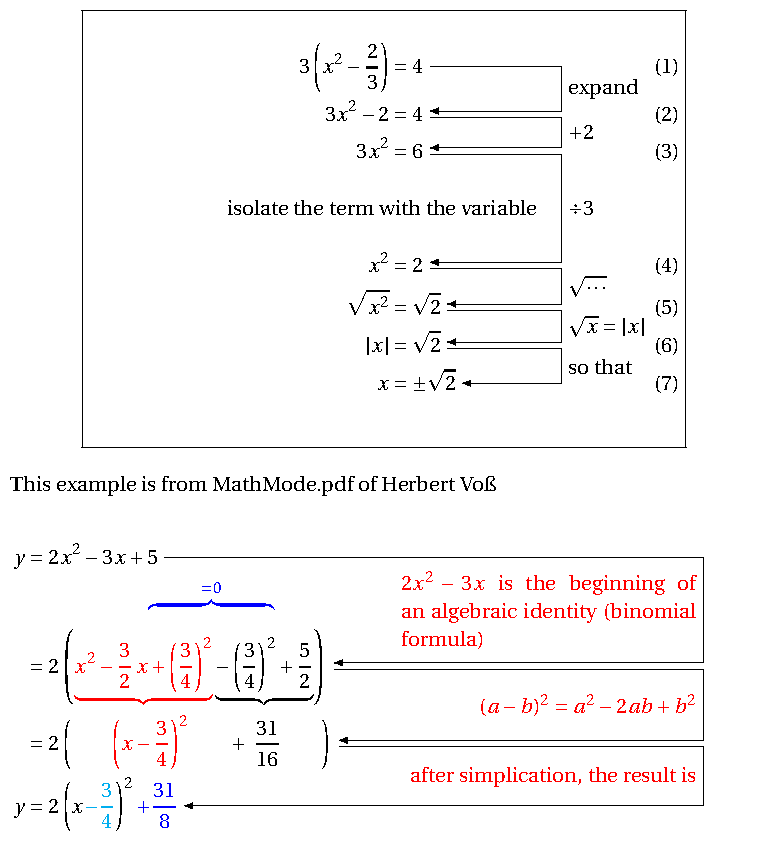
\includegraphics[width=0.45\textwidth]{tkz-linknodes-examples}}
\newlength\alturaA
\settoheight\alturaA{\usebox{\exemploA}}

\newsavebox\exemploB
\savebox\exemploB{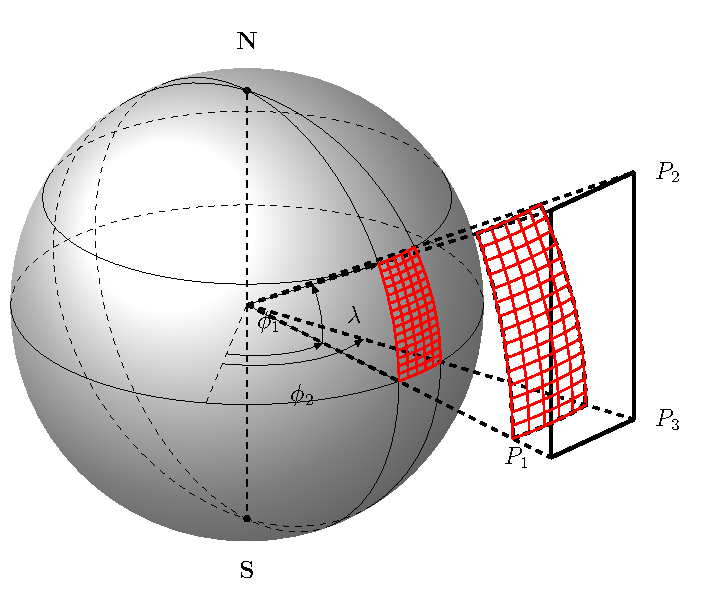
\includegraphics[width=0.45\textwidth]{spherical-and-cartesian-grids}}
\newlength\alturaB
\settoheight\alturaB{\usebox{\exemploB}}

\subsection{O pacote TikZ}
\begin{frame}
	\frametitle{TikZ}
	\framesubtitle{\href{http://sourceforge.net/projects/pgf/}{http://sourceforge.net/projects/pgf/}}
		
	\begin{columns}
		\column{0.45\textwidth}
		\begin{block}{Exemplo 1}
			\usebox{\exemploA}
		\end{block}
		
		\column{0.45\textwidth}
		\begin{block}{Exemplo 2}
			\rule[0.5\alturaB-0.5\alturaA]{0pt}{\alturaA}\usebox{\exemploB}
		\end{block}
	\end{columns}

	\vfill

	\begin{center}
		\footnotesize
		Outros exemplos: \href{http://www.texample.net/tikz/examples/}{http://www.texample.net/tikz/examples/}
	\end{center}
	
\end{frame}
%-------------------------------------------------------------------
\savebox\exemploA{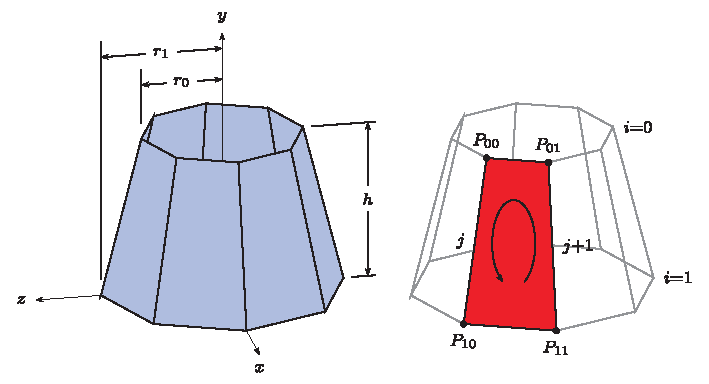
\includegraphics[width=0.45\textwidth]{piramide}}
\settoheight\alturaA{\usebox{\exemploA}}
\savebox\exemploB{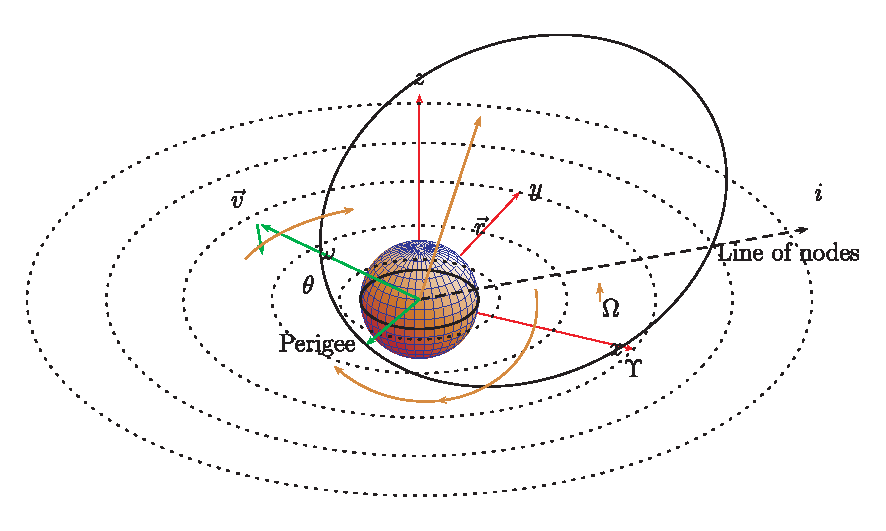
\includegraphics[width=0.45\textwidth]{orbita}}
\settoheight\alturaB{\usebox{\exemploB}}

\subsection{O pacote pstricks}
\begin{frame}
	\frametitle{PSTricks}
	\framesubtitle{\href{http://www.tug.org/PSTricks/}{http://www.tug.org/PSTricks/}}
	
	\begin{center}
		Exclusivamente para documentos PostScript, embora o perfil $\text{\LaTeX} \Rightarrow \text{PS} \Rightarrow \text{PDF}$ possa ser utilizado para produzir PDF
	\end{center}
	
	\begin{columns}
		\column{0.45\textwidth}
		\begin{block}{Exemplo 1}
			\rule[-0.5\alturaB+0.5\alturaA]{0pt}{\alturaB}\usebox{\exemploA}
		\end{block}
		
		\column{0.45\textwidth}
		\begin{block}{Exemplo 2}
			\usebox{\exemploB}
		\end{block}
	\end{columns}

	\vfill

	\begin{center}
		\footnotesize
		Outros exemplos: \href{http://www.tug.org/PSTricks/main.cgi?file=examples}{http://www.tug.org/PSTricks/main.cgi?file=examples}
	\end{center}
	
\end{frame}
%-------------------------------------------------------------------
\section{Papel de parede ou marca d'água}
\begin{frame}[fragile]
	\frametitle{Papel de parede ou marca d'água}
	
	\begin{atividade}<1->{9: através do pacote \pkg{wallpaper}}
		\begin{tabbing}
			\cs{ThisCenterWallPaper}\=\{\textit{fator de escala}\}\{\textit{arquivo da figura}\}\kill
			\>\cs{CenterWallPaper}\'\{\textit{fator de escala}\}\{\textit{arquivo da figura}\}\\
			\cs{ThisCenterWallPaper}\{\textit{fator de escala}\}\{\textit{arquivo da figura}\}
		\end{tabbing}
	\end{atividade}
	
	\vfill
	
	\begin{atividade}<2->{10: através do pacote \pkg{tikz}}
		\begin{LaTeXcode}
		\begin{tikzpicture}[remember picture,overlay]
		  \node [opacity=0.50] at (current page.center)
		    {\includegraphics[height=\paperheight,width=\paperwidth]
		      {./figuras/Tei-Gi_a4paper}};
		\end{tikzpicture}
		\end{LaTeXcode}
	\end{atividade}
	
	\vfill
	
	\begin{center}
		\footnotesize
		\textbf{obs.:} o leão-pensador nas listas de exercício foi inserido através\\do pacote \pkg{wallpaper}, como acima.
	\end{center}
	
\end{frame}
%-------------------------------------------------------------------
\ifhandout\else
{
	\logo{
\includegraphics[width=0.25\textwidth]{LogotipoCursoLaTeX_v3_pequeno}}
	\setbeamertemplate{background canvas}{}
	\againframe{titulo} % Reapresenta a página inicial.
}
\fi
%-------------------------------------------------------------------
%-------------------------------------------------------------------
%-------------------------------------------------------------------
\appendix
\section{Respostas}
\begin{frame}[fragile,label=respostas]
	\frametitle{Respostas dos exercícios}

	\footnotesize

	\begin{enumerate}
	\item O primeiro espaço é dado pelo comando \verb*|\ | e o segundo, pela quebra de linha logo após o \cs{includegraphics}.
	\item%
		\begin{LaTeXcode}
			\begin{figure}			  
			  \begin{minipage}{0.45\textwidth}
			  	\includegraphics[width=\textwidth]{...}
			  	\caption{...}
			  \end{minipage}\hfill
			  \begin{minipage}{0.45\textwidth}
			  	\includegraphics[width=\textwidth]{...}
			  	\caption{...}
			  \end{minipage}
			\end{figure}
		\end{LaTeXcode}
		
		\textbf{obs.:} a soma da largura das duas minipáginas deve ser inferior à largura da linha e, preferencialmente, menor que ela.
	\end{enumerate}

\end{frame}
\end{document}